\chapter{The \acs{LHC} and the \acs{CMS} experiment}
\label{chap:CMSLHC}

\section{The \acs{LHC}}
\label{sec:CMSLHC_LHC}

The \acf{LHC} \cite{lhc-machine}  is a 26.7 km long synchrotron hadron accelerator and collider below the surface of the 
Franco-Swiss border near Geneva. It
is installed in the tunnel that previously housed the Large Electron Positron accelerator
that was operated by \acf{CERN} between 1989 and 2000.

The \ac{LHC} was designed to collide beams of protons with each other at centre-of-mass
energies of up to 14 TeV. It therefore consists of two rings in which the two beams
of protons are individually accelerated. In addition to colliding beams of protons, the \ac{LHC}
is also used for proton--lead and lead--lead collisions.

The \ac{LHC} does not operate on its own, a chain of accelerators leads
the protons into the \ac{LHC}. Figure \ref{fig:lhc_schematic} shows a schematic
of the \ac{CERN} accelerator complex.
\begin{figure}[h!]
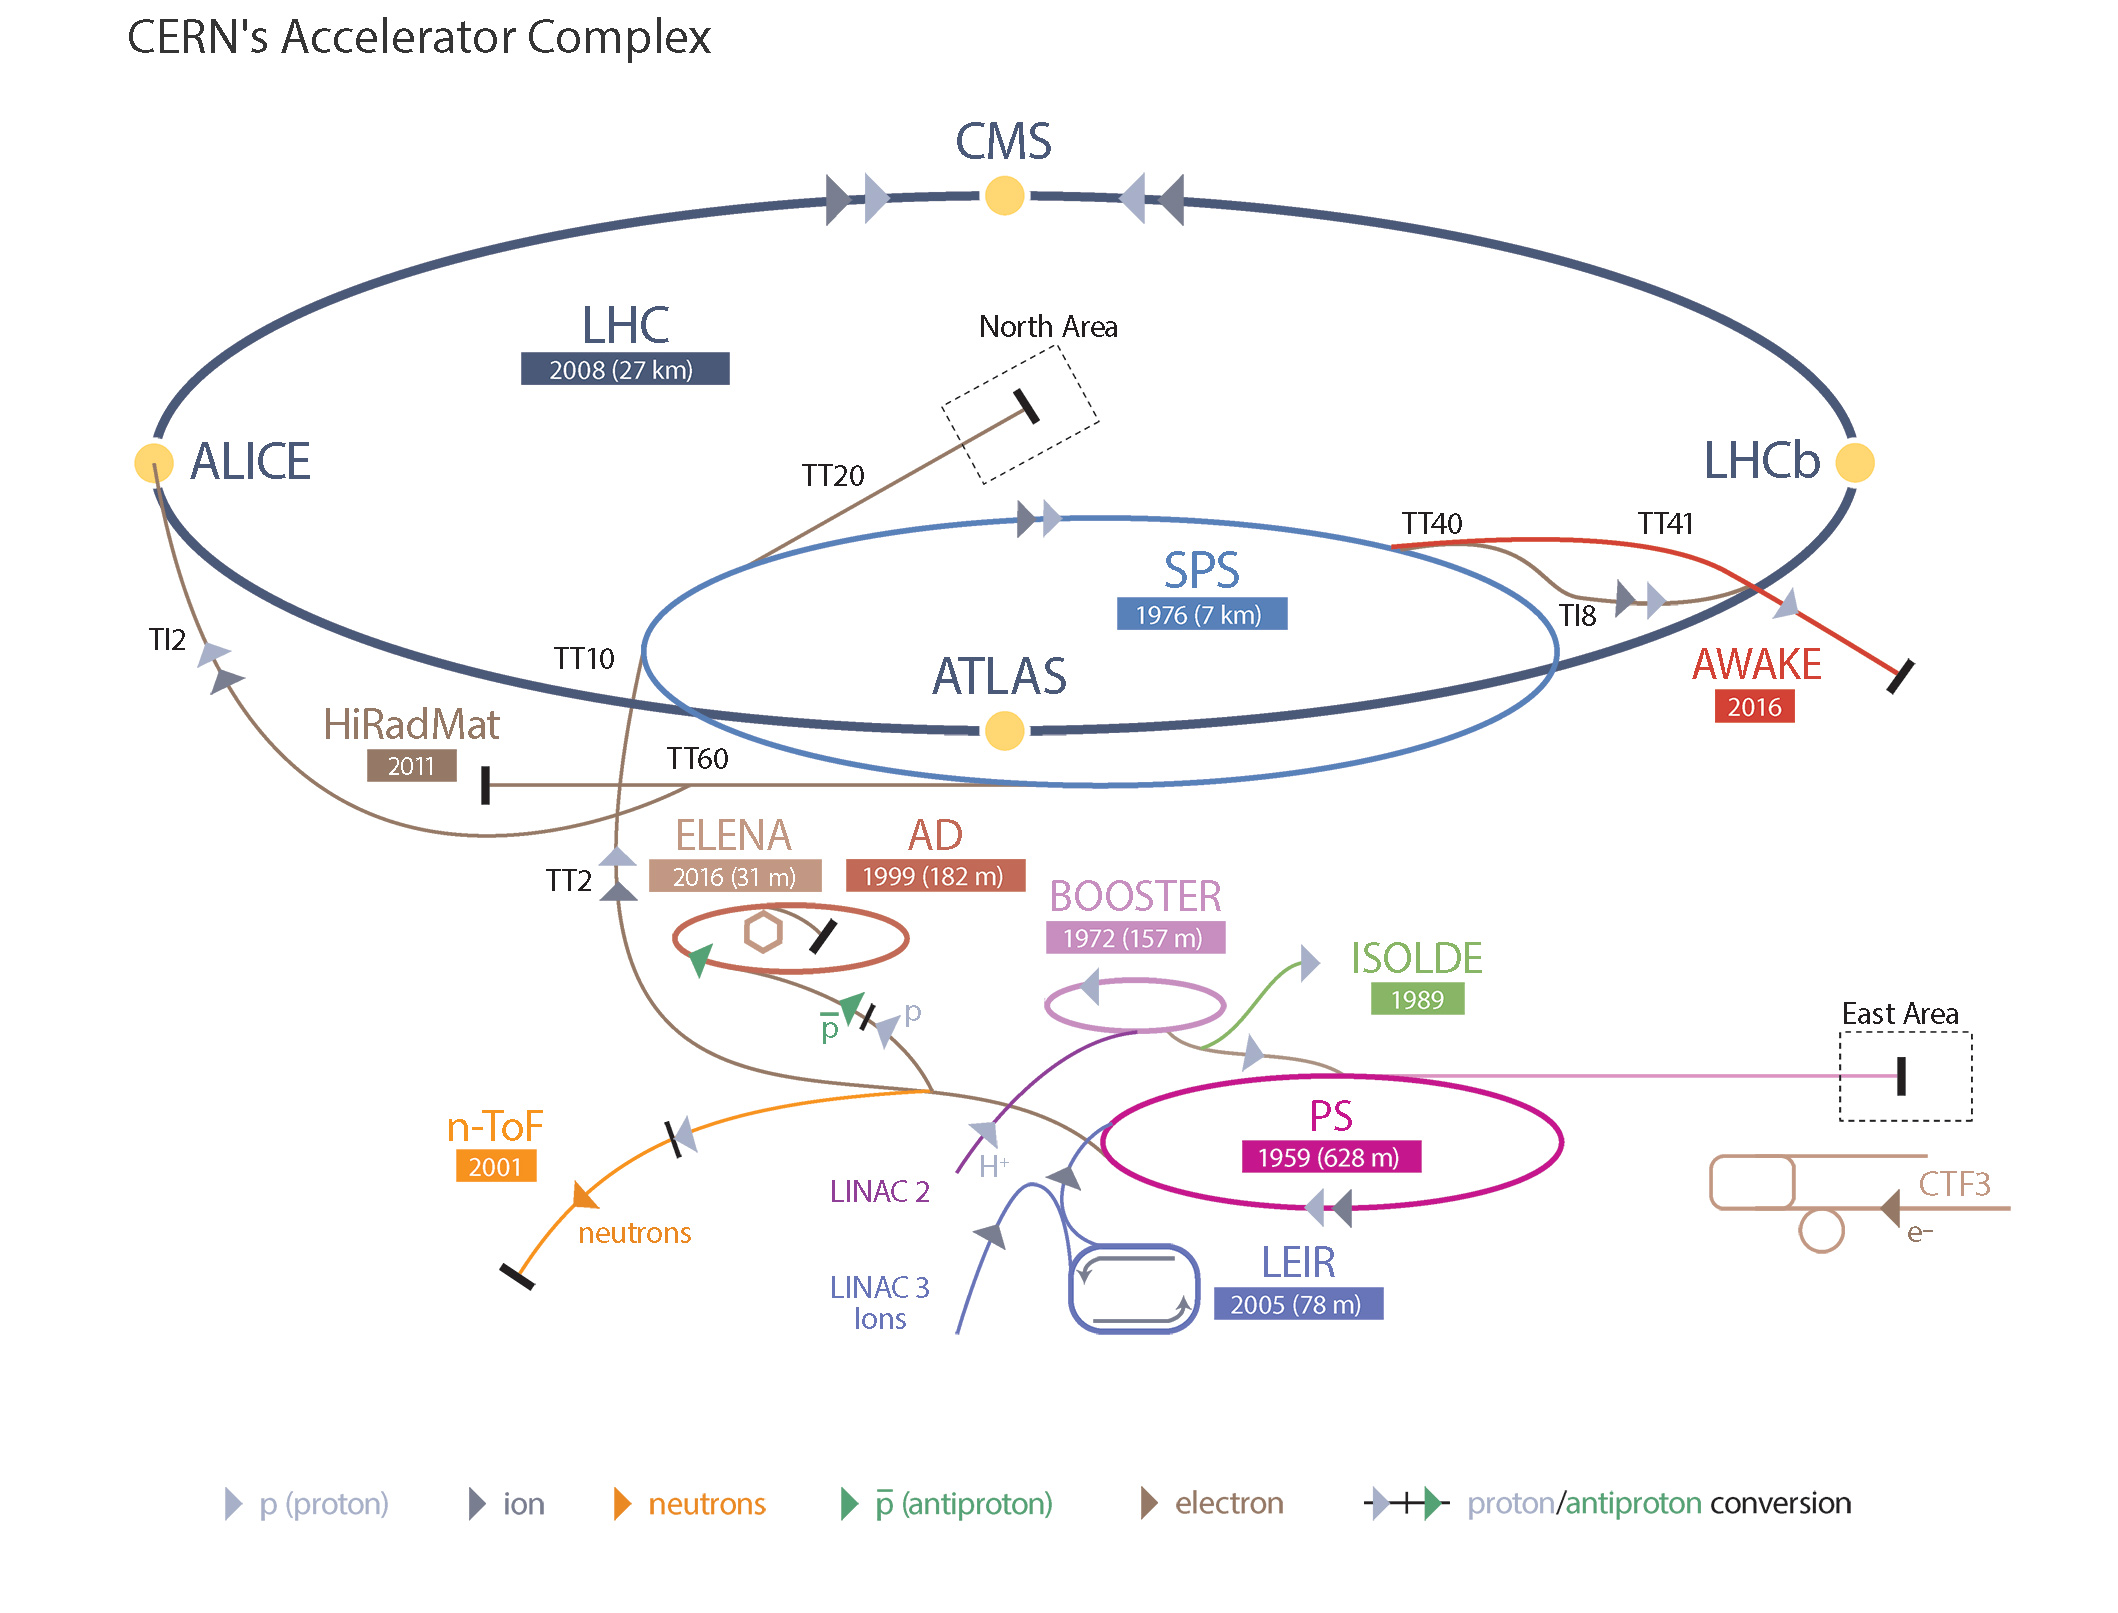
\includegraphics[width=0.8\textwidth]{./Detector/Plots/LHC_default.jpg}
\caption{Schematic of the \ac{CERN} accelerator complex \cite{lhc-schematic}.}
\label{fig:lhc_schematic}
\end{figure}
Protons originate from hydrogen gas, where electrons are stripped off the 
hydrogen atoms using an electric field. The protons then pass through an injector
chain which increases the energy of the protons in several steps. After the protons
are created from the hydrogen gas, they are accelerated to a centre of mass energy of
50 MeV in the Linac2 linear accelerator. They are then passed on to the
\acf{PSB} which accelerates the protons until they reach a centre of mass energy of 1.4 GeV.
The next accelerator in the chain, the \acf{PS}, further accelerates the protons to 25 GeV,
with the \acf{SPS} bringing the energy up to 450 GeV. When this energy has been 
reached the protons are injected into the \ac{LHC} in two counter-rotating
beams. In the \ac{LHC} ring the beams are further accelerated to the required centre of mass energy
by eight \ac{RF} cavities. At design operation the beams consist of 2808 proton bunches each made up 
of $\mathcal{O}(10^11)$ protons, spaced 25ns apart. The beams are kept in circulation
using 1232 niobium-titanium superconducting dipole magnets, cooled to operate at 
a temperature of 1.9K and generating magnetic fields upwards of 8 T.
The beams collide at four points
around the \ac{LHC} ring, where the collisions are recorded by the ATLAS\cite{atlas-jinst}, 
CMS%\cite{cms-jinst} guess we've cited this already
, ALICE\cite{alice-jinst}, and LHCb\cite{lhcb-jinst} detectors.

The processes the \ac{LHC} was built to study have a small cross-section
compared with the total proton-proton inelastic cross-section, as seen from figure
\ref{fig:stirling_xs}. For example, the production cross-section of the
standard model Higgs boson is 9-10 orders of magniuted smaller than the total p--p cross section.

\begin{figure}[h!]
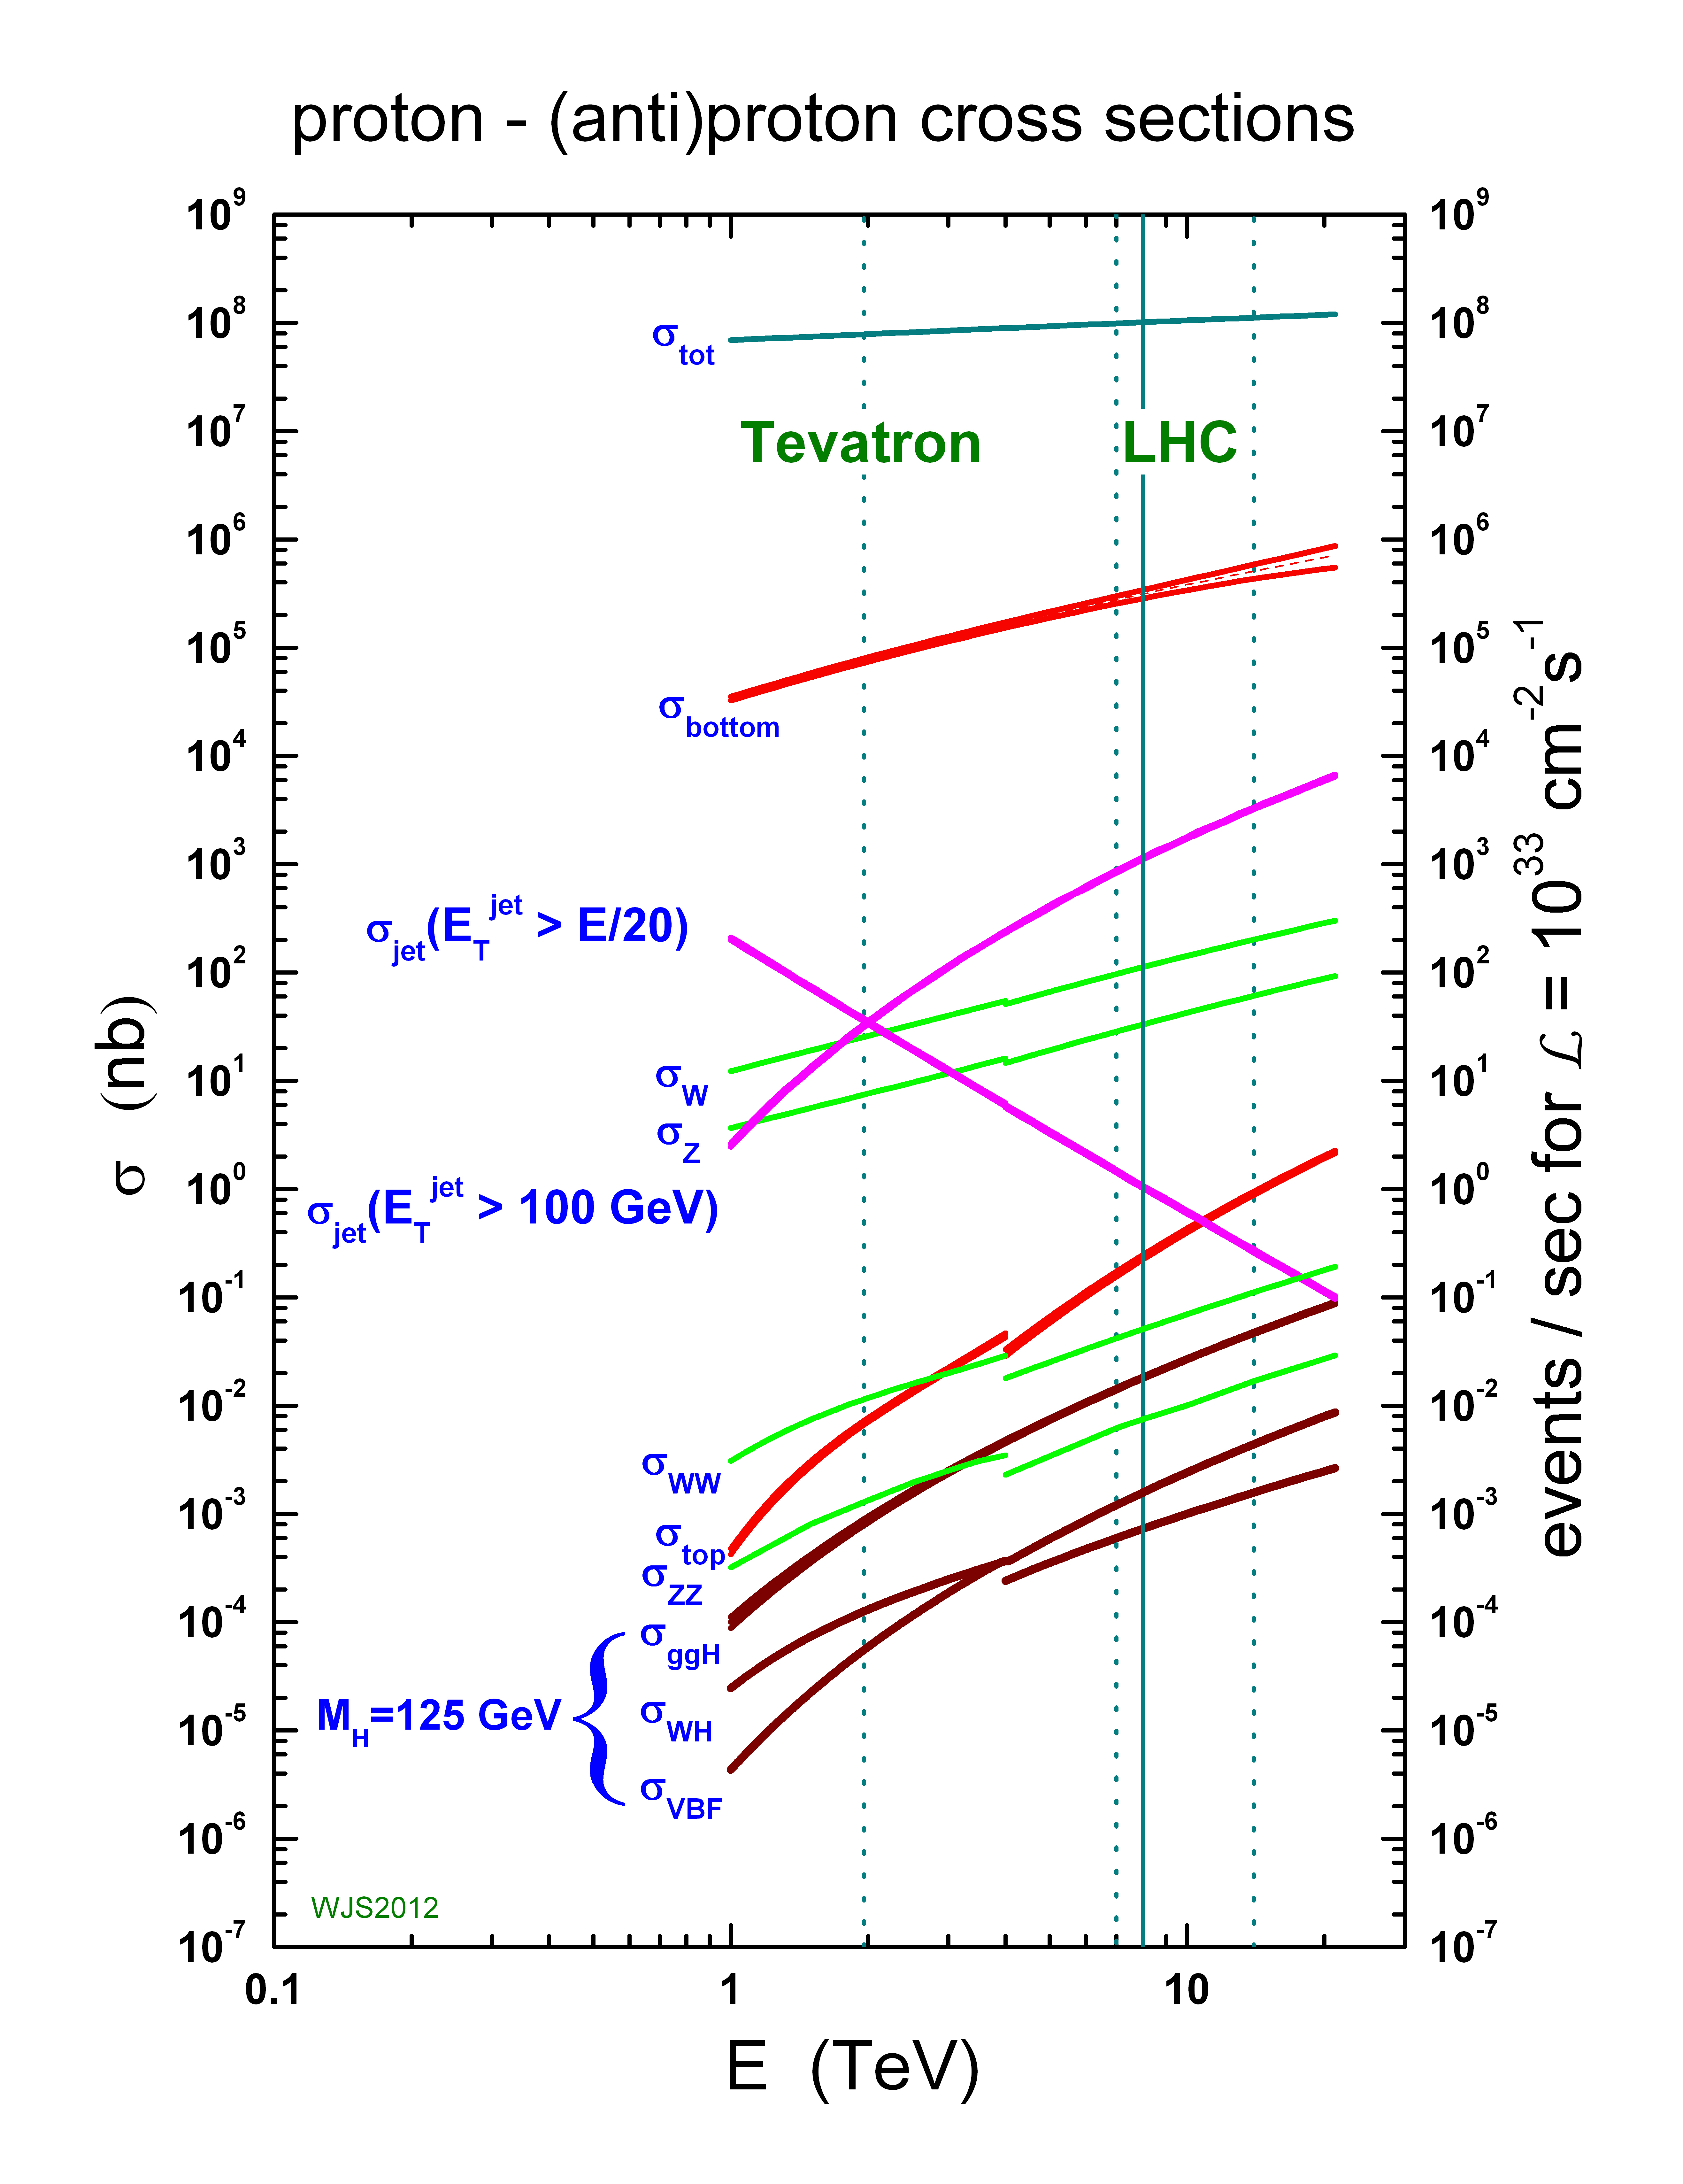
\includegraphics[width=0.5\textwidth]{./Detector/Plots/crosssections2013.jpg}
\caption{Total proton-proton cross section, and the cross-sections
for several processes studied at the LHC \cite{stirling-crosssection}.
The cross sections of these processes
are often many orders of magnitude smaller than the total p--p cross section.}
\label{fig:stirling_xs}
\end{figure}

In order to be able to study these relatively rare processes, 
the LHC operates at high instantaneous luminosity, defined as
\ref{eqn:CMSLHC_luminosity}. 
\begin{equation}\label{eqn:CMSLHC_luminosity}
\mathcal{L} = \frac{N_b^2n_bf_{\text{rev}}\gamma}{4\pi\epsilon_n\beta^{*}}F.
\end{equation}

In this equation, $N_b$ is the number of protons per bunch, $n_b$ the number of
bunches per beam, $f_{\text{rev}}$ the revolution frequency, $\gamma$ the 
Lorentz factor, $\epsilon_n$ the normalised beam
emittance, $\beta^{*}$ the $\beta$-function at the interaction point and F a reduction
factor due to the crossing angle. 

After an initial testing phase, the \ac{LHC} began its first physics run in May 2010 with 
a centre of mass energy of 7 TeV. The CMS experiment recorded an integrated luminosity of 45 pb$^{-1}$
during 2010. In 2011 the \ac{LHC} continued operating at a centre-of-mass energy of 7 TeV, delivering an integrated 
luminosity of 6.1 fb$^{-1}$ to the CMS experiment. The centre of mass energy was increased to 8 TeV
for the 2012 data-taking period, during which an integrated luminosity of 23.3 fb$^{-1}$ was delivered.
This completed Run 1 of the \ac{LHC}, after which the 2-year \ac{LS1} was used to 
upgrade the LHC and the detectors for collisions at a centre of mass energy of 13 TeV.

In April 2015 the \ac{LHC} restarted with collisions at a centre-of-mass energy of 13 TeV, and during 
this year 4.2 fb$^{-1}$ was delivered. Collisions at a centre-of-mass energy of 13 TeV continued
in 2016, when a total of 41.1 fb$^{-1}$ was delivered. 
The integrated luminosity as a function of time is shown in figure \ref{fig:CMSLHC_intlumi},
separated by running year.

\begin{figure}[h!]
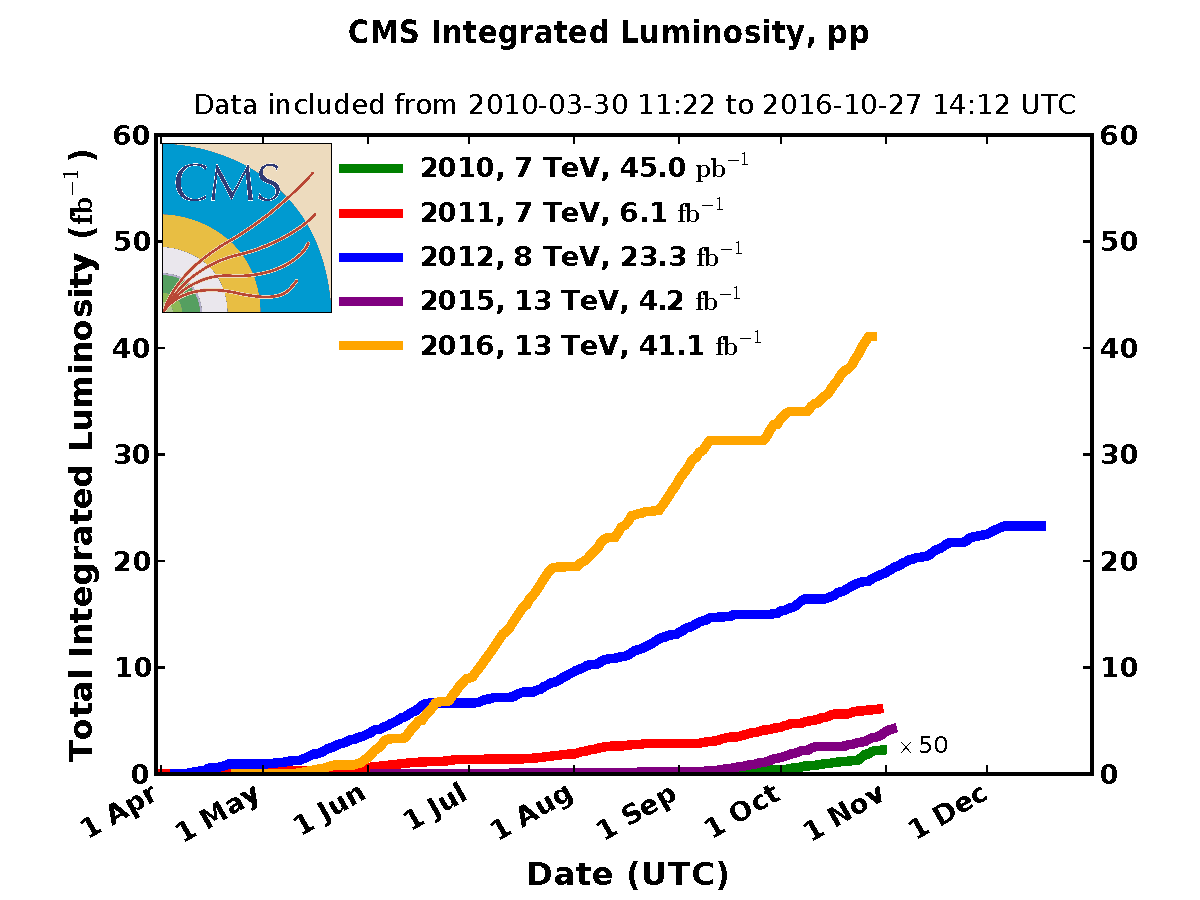
\includegraphics[width=0.85\textwidth]{./Detector/Plots/int_lumi_cumulative_pp_2.pdf}
\caption{Cumulative integrated luminosity for p--p collisions at the LHC, separated
by running year \cite{cms-lumi-public}.}
\label{fig:CMSLHC_intlumi}
\end{figure}

The data-taking efficiency of CMS is not 100\%, for example the detector might be
switched off for part of the time collisions are ongoing. In 2012, the data-taking 
efficiency was 93.5\%, in 2015 it was 90.3\% and in 2016 it was 92.4 \%

From all of the data that is recorded, a subset is used for analyses. Data is 
certified as good for use in analyses if it is known that all relevant subdetectors
were functioning correctly. The certification efficiency in 2012 was 90.4\%,
leading to an integrated luminosity of 19.7 fb$^{-1}$ for which all subdetectors
were working well, in 2015 it was 60.4 \%, leading to 2.3 fb$^{-1}$ of analysable data
for which the full detector was operational. An additional 0.6 fb$^{-1}$ was taken
with the magnet switched off. The certification efficiency for the full 2016 p--p running period was 95.4\%.

The \ac{LHC} was designed for a nominal
peak luminosity of $10^{32}$cm$^{-2}$s$^{-1}$ for proton-proton collisions. In 2012 peak
luminosities of $7.7*10^{33}$cm$^{-2}$s$^{-1}$ were reached, with the peak luminosity in
2015 being $5.1*10^{33}$cm$^{-2}$s$^{-1}$. Since July 2016
the \ac{LHC} has been operating at instantaneous luminosities upwards of the 
design luminosity, with peak luminosities of $1.5*10^{32}$cm$^{-2}$s$^{-1}$ reached
in October 2016.

Due to the high operating luminosity, multiple proton-proton collisions per 
bunch crossing are likely to occur. The average number of interactions
per bunch crossing was 21 in 2012\cite{cms-lumi-public}. The average number of
interactions per bunch crossing lowered again at the start of Run 2, with
an average of 14 interactions per bunch crossing for the data collected
during 2015. In the data-taking period up to August 2016 the average number of interactions
per bunch crossing increased to 24\footnote{NoteToBeRemovedBeforeSubmission: Lumi pog letting us down 
here, no references for what number to quote/no prescriptions for how to calculate it. Use of theoretical
min bias cross section (80mb) vs min bias cross section tuned for pu reweighting (less than 70 mb both for
2015 and 2016) can shift the average by 5 evts or more! The 2016 number uses the theoretical
cross section (only reference to this are various sets of slides presented at conferences), 2015
number based on the min bias cross section used for pu reweighting (iirc). Assuming the 2012 numer,
for which there is a public figure, uses the theoretical mb cross section should probably re-calculate the
number for 2015.}. Additional 
interactions on top of events of interest are referred to as pile-up.

\section{The \acs{CMS} detector}
\label{sec:CMSLHC_CMS}
To meet the demands of the \ac{LHC} physics programme, the
 \ac{CMS} detector was designed to be very perfomant in searches
for physics at the TeV scale and to be able to 
function in the challenging high-luminosity environment.
The detector is 21.6 m long, 14.6 m in diameter, and weighs
12500 tonnes \cite{cms-jinst}. It consists of several subdetectors, as illustrated
in figure \ref{fig:cms_detector}. Surrounding the interaction
point is the silicon tracker, a cylinder 5.8 m in lenght and 2.6 m in 
diameter. Surrounding the silicon tracker
the lead-tungstate \ac{ECAL} is found, which in turn is enclosed
by a brass scintilator \ac{HCAL}. 

The tracking and calorimeter systems are surrounded by a superconducting
solenoid, 13 meter long and 6 meter in diameter and operating at 3.8 Tesla.
Charged particles are bent in this magnetic field, allowing for precise 
measurement of their momentum. Gaseous muon detectors are embedded in the 
iron return yoke of the solenoid.

For the measurement of physical quantities, \ac{CMS} uses a coordinate
system with the origin centred at the nominal collision point
inside the experiment. The y-axis points vertically upward, the x-axis
points radially inward toward the centre of the \ac{LHC} ring. The z-axis
points along the beam direction. As such the transverse momentum and energy, 
\pT and \ET are measured from the x- and y- components of the momentum and energy.
The azimuthal angle $\phi$ is measured in the x-y plane with respect to the x-axis, 
the polar angle $\theta$ measured with respect to the z-axis. A coordinate
more frequently used than the polar angle is the pseudorapidity $\eta = -\ln{[\tan{\frac{\theta}{2}}]}$.
Distances in the $\eta-\phi$ plane are given as $\Delta R = \sqrt{(\Delta\eta)^2+(\Delta\phi)^2}$. 

The subsystems of the \ac{CMS} detector will be described in more detail in the 
next sections.

\begin{figure}[h!]
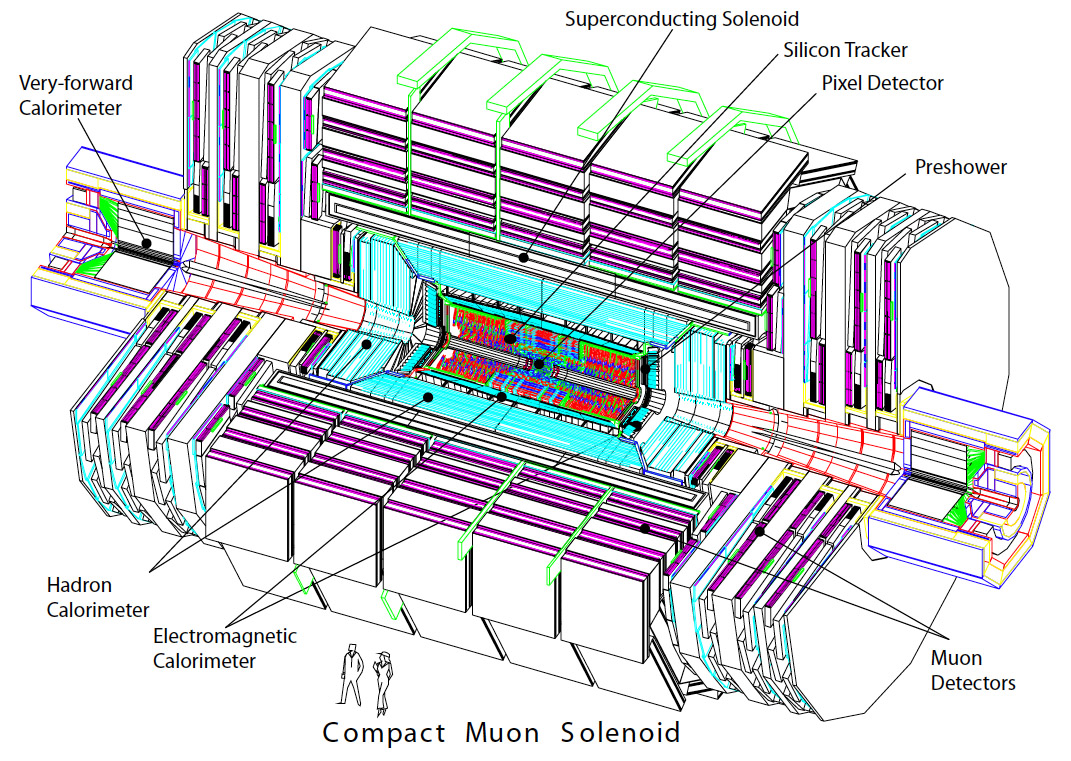
\includegraphics[width=0.8\textwidth]{./Detector/Plots/cms.png}
\caption{A blow-up view of the \ac{CMS} detector \cite{cms-jinst}, indicating the
different sub-parts of the detector.}
\label{fig:cms_detector}
\end{figure}

\subsection{Tracker}
\label{sec:CMSLHC_CMS_tracker}
The tracker \cite{cms-jinst} is the subdetector closest to the interaction point. It
is used for accurate reconstruction of charged particle trajectories and 
the precise reconstruction of secondary vertices, which are important to be
able to indentify heavy-flavour particles. This means a small impact parameter
resolution needs to be achieved, for which a highly granular system is required. 
Due to the large number of particles emerging from 
each collision, an average of 1000 per bunch crossing (every 25 ns) at LHC design operation, the 
system also needs to be fast-responding in order to reconstruct trajectories accurately.
At the same time, this large particle flux calls for a 
radiation-hard design that is able to survive in this harsh environment
for a longer period of time. These requirements motivate the use of a silicon tracking
system. When a charged particle passes through the silicon, an electron-hole pair
is created, which drift under an applied electric field and produce a current
that can be read out. %LEARN A BIT MORE ABOUT THIS

The tracker provides coverage up to $|\eta| < 2.5$ and consists of
several different components. A schematic of the tracking detector is given
in figure \ref{fig:CMS_tracker}. The part of the tracking system
closest to the interaction point is the silicon pixel detector, which 
consists of 3 layers of pixels in the barrel of the detector, with 
2 pixel endcap disks. The barrel layers sit at radii of 4.4, 7.3 and 10.2 cm 
and extend up to $z=\pm 26.5$ cm, with the disks placed at $z=\pm 34.5$ cm and
$z=\pm 46.5$ cm. The pixel detector consists of 66 million silicon pixels, each
$100 \mu m \times 150 \mu m$ in size. The choice of this pixel size is driven
by the achievable spatial resolution, which is $15-20 \mu m$ in the $r$ and $z$ directions.
This allows for 3D vertex reconstruction. With this layout, the pixel tracker
provides 3 precise position measurements along each charged particle trajectory.


\begin{figure}[h!]
\begin{center}
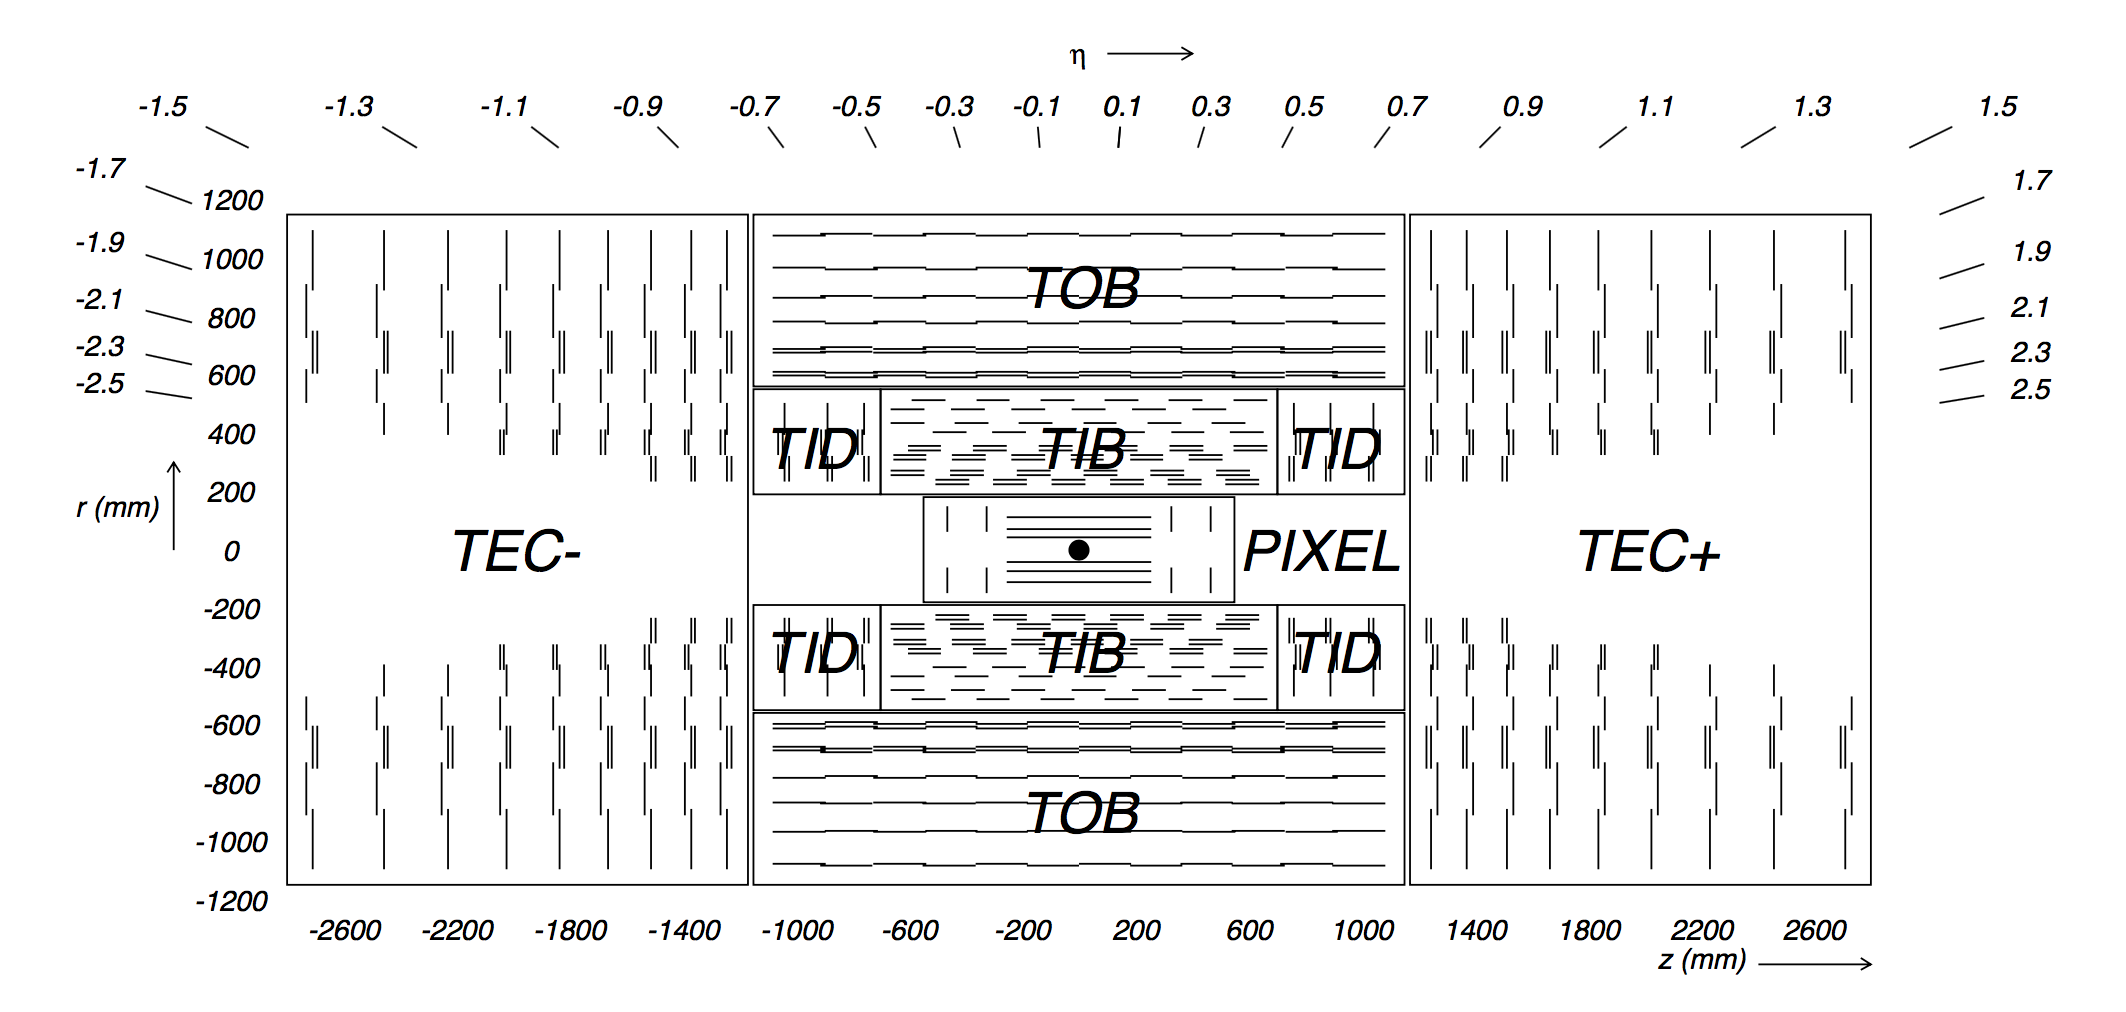
\includegraphics[width=0.9\textwidth]{./Detector/Plots/Tracker.png}
\caption{Schematic of the CMS tracker in the r-z plane, indicating the
positions of the pixel and strip detectors \cite{cms-jinst}. Each line 
on the plot represents a detector module}
\label{fig:CMS_tracker}
\end{center}
\end{figure}


Beyond the pixel detector the tracking system is made up of a silicon
strip detector consisting of over 9 million multiple different subsystems. The first part of the
silicon strip tracker consists of \ac{TIB} and \ac{TID}, providing 4 layers of
silicon strip detectors in the barrel plus 3 disks at both ends. These two systems
extend out towards a radius of 55 cm. The barrel layers and disks each consist
of silicon strips which are 10 cm long, $80-141\mu m$ wide and $320 \mu m$ thick. The \ac{TIB} and \ac{TID}
provide 4 measurements of the $r-\phi$ position  with a resolution of 23-35 $\mu m$.
The \ac{TIB} and \ac{TID} are surrounded by the \ac{TOB}, which consists of 6 layers of silicon strip sensors extending
up to an outer radius of 116 cm and up to $z=\pm 118$ cm. The strips in the \ac{TOB} are 500 $\mu m$ thick, around 25 cm long and 122-183 $\mu m$ 
wide and this subdetector provides 6 measurements of $r$ and $\phi$, with a resolution
of 35-53 $\mu m$. Beyond the z-range covered by the \ac{TOB}, coverage is provided by the \ac{TEC},
consisting of 9 disks of strips.In the \ac{TEC}, the thickness ranges from 320-500 $\mu m$ and the the strip width ranges from $97-184 \mu m$.
In this way this part of the system provides up to 9 $\phi$ measurements.

Some of the strip modules in the detector carry a second strip detector module mounted back-to-back with a stereo angle %FIXME WTF?
of 100 mrad, in order to provide measurements of the $z-$ coordinate in the barrel. This is achieved with a resolution of 230-530 $\mu m$.

The pixel tracker will be upgraded during the extended year-end technical stop in early 2017. %or just replaced?


\subsection{\acl{ECAL}}
\label{sec:CMSLHC_CMS_ecal}
The \ac{ECAL} \cite{cms-jinst} is a hermetic homogeneous calorimeter
made of nearly 76000 lead tungstate (PbWO$_4$) crystals. It has very
good energy resolution, is highly granular and fast-responding, which
are all needed to be able to detect $H\rightarrow \gamma\gamma$ decays.

Despite being further away from the interaction
point than the tracker, the materials in other parts of the detector
still need to be radiation hard. In order to be able to place
the calorimeters inside the bore of the solenoid, a compact \ac{ECAL}
had to be constructed, and to provide excellent resolution a 
highly granular system had to be designed. The lead tungstate crystals have a 
radiation length of 0.89 cm, a Moli\`ere radius of 2.2 cm, and 80\% of the light
from the crystals is emitted in 25 ns. This short radiation
length, small Moli\`ere radius and short scintillation decay time combined
with the radiation hardness of the material motivate the choice of lead tungstate. 

%Moliere radius: characteristic constant of a material giving scale of transverse dimenstion
%of fully contained EM showers. It is the radius of a cylinder containing on average 
%90pct of the shower's energy deposition. Related to radiation length as 
%molrad approx 0.0265X0 (Z+1.2) with Z the atomic number.
%Radiation length: mean distance over which a high energy electron
%loses all but 1/e of its energy by bremmstrahlung and 7/9 of th emean free path for pair production by 
%a high energy photon.

When a high energy electron or photon enters a crystal, it starts a
shower producing a cascade of lower energy particles. Electrons lose
energy through bremsstrahlung, with photons undergoing $\Pe^+ \Pe^-$ 
pair production. The shower continues until the photon energy drops below the 
$\Pe^+\Pe^-$ pair production threshold, and ionisation 
starts to dominate for electrons. The shower ionises the crystals, 
which return to their normal state by emitting scintillation light. 
As the crystals are 25.8 radiation lengths long, most of the shower
is contained inside them.

Figure \ref{fig:CMS_ECAL} shows a schematic of the \ac{ECAL}, indicating
the geometry. The \ac{ECAL} consists of different subsystems. The \ac{EB} 
covers the pseudorapidity range up to $|\eta|<1.479$, with
crystals of $0.0174 \times 0.0174$ in $\eta - \phi$. The \ac{EE}
provides coverage beyond the range of the \ac{EB}, up to $|\eta|<3.0$
Each endcap is divided into two halves. In front of the endcaps 
the preshower detectors, covering $1.653<|\eta|<2.6$ is a sampling
calorimeter whose main use is to indentify neutral pions in the endcaps. Additionally
it helps electron identification and improves the resolution
of position determination. Each of the two preshower detectors consist
of two layers of lead radiators to initiate the shower, with silicon sensors
placed after each layer of radiators to measure the deposited energy. The 
total thickness of the preshower comprises 3 radiation lenghts.

\begin{figure}[h!]
\begin{center}
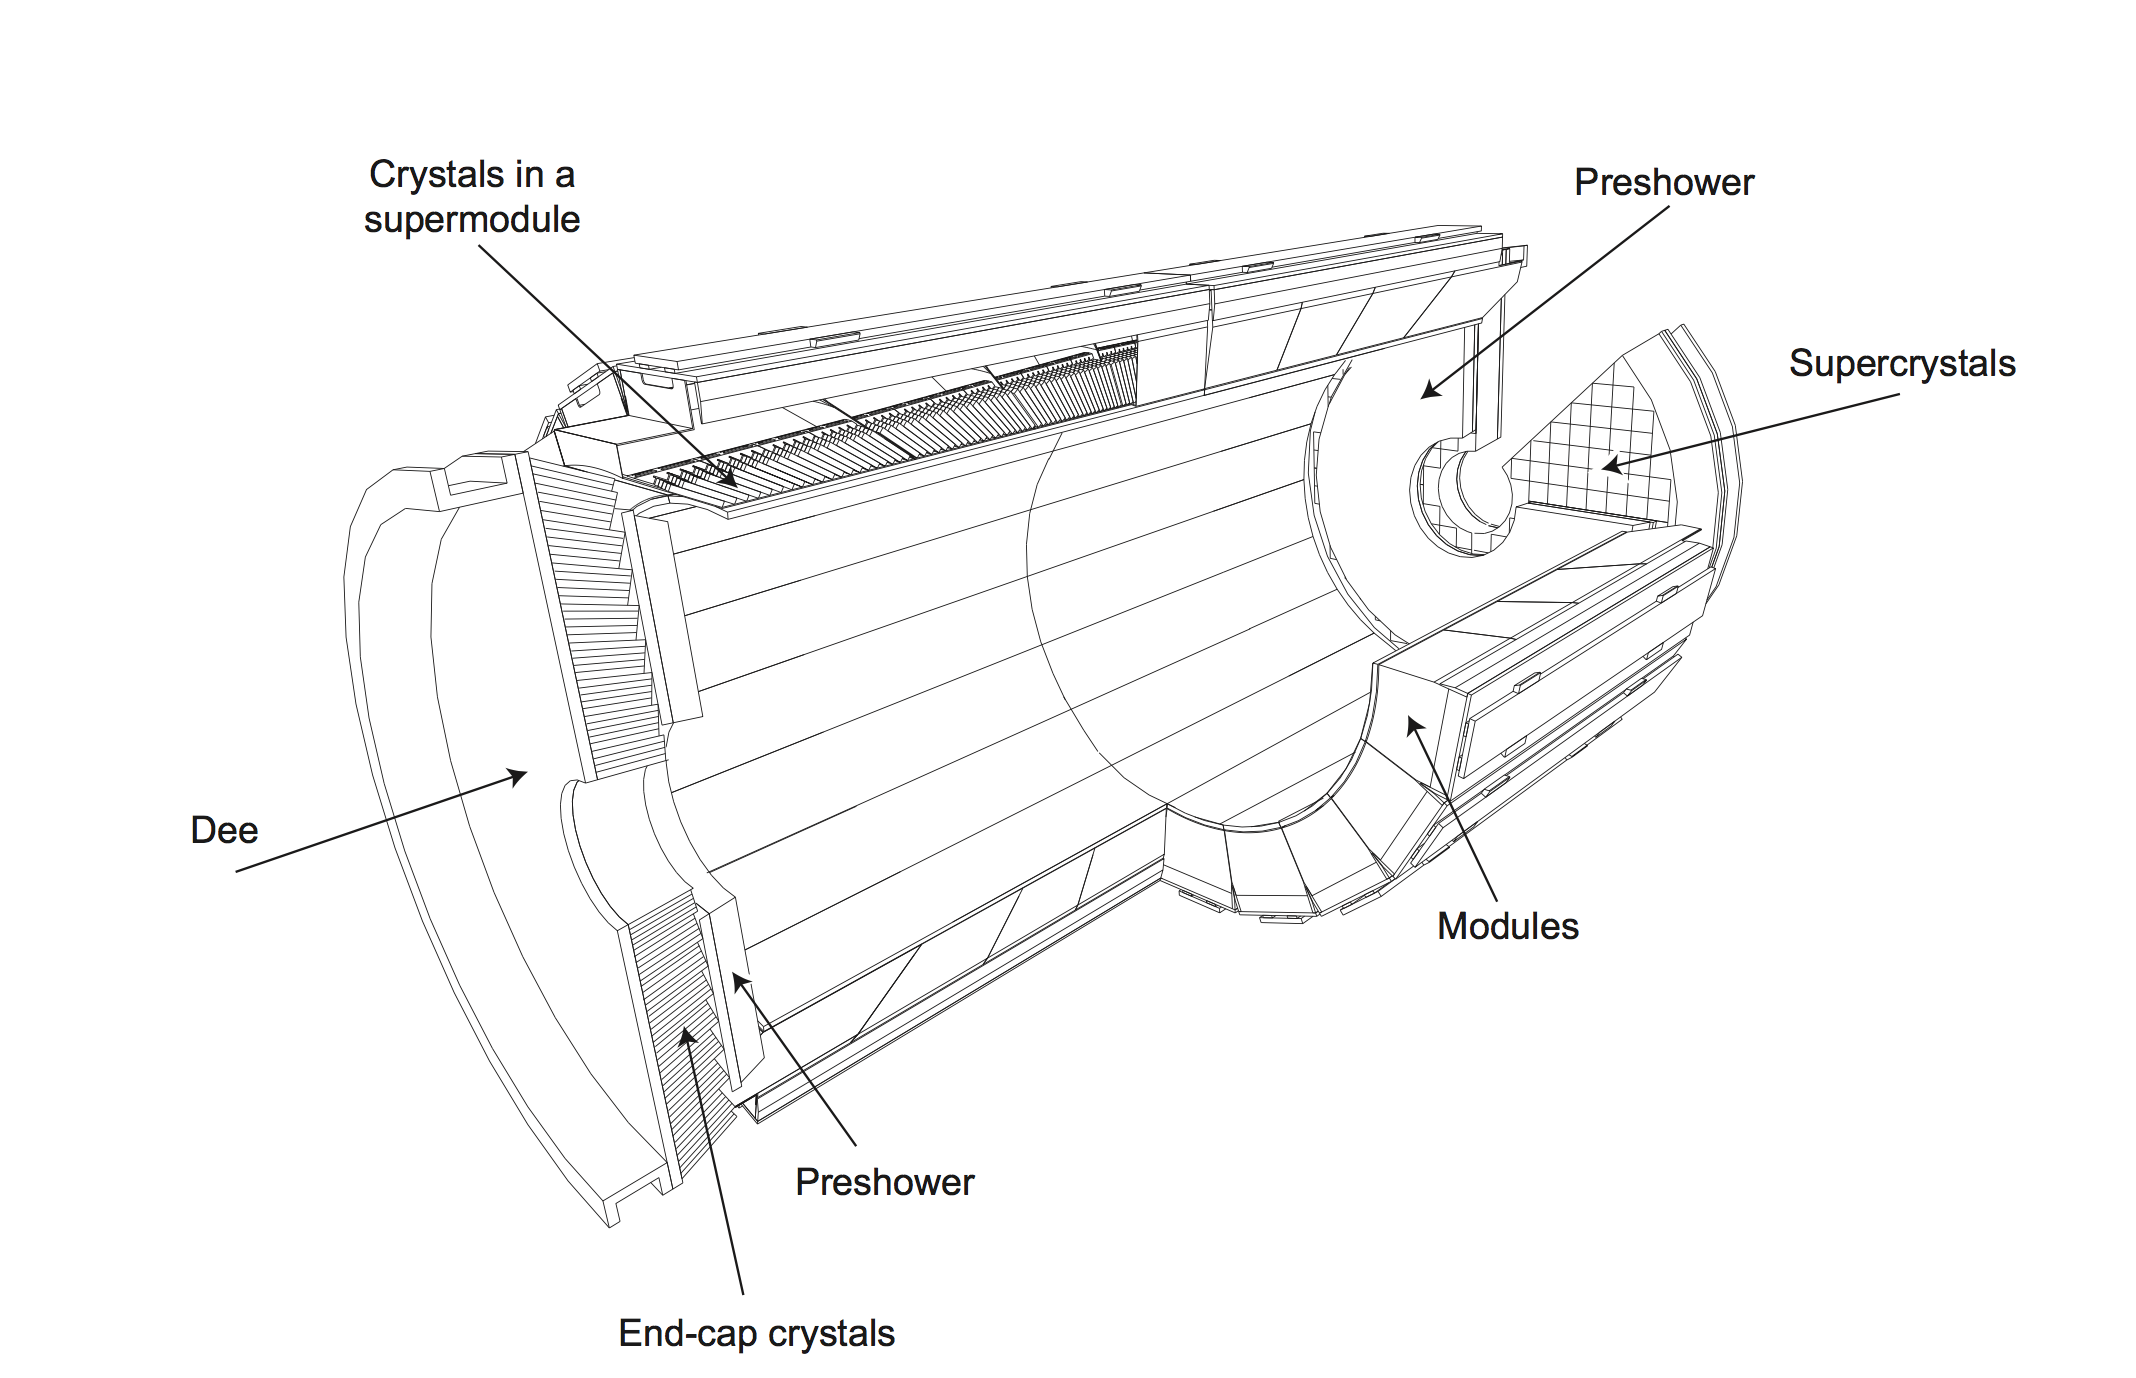
\includegraphics[width=0.9\textwidth]{./Detector/Plots/ECAL.png}
\caption{Layout of the \ac{ECAL}, indicating the position of the
different components \cite{cms-jinst}.}
\label{fig:CMS_ECAL}
\end{center}
\end{figure}

To preserve the energy resolution, the \ac{ECAL} crystal and
photodetector temperatures need to be kept stable within $\pm 0.05^o$C
as the number of scintillation photons emitted by the crystals,
and the amplification of the photodetectors are temperature dependent.
The nominal operating temperature, $18^o$C, is ensured by 
supplying the detector with water at this temperature.

To record the light yield of the crystals, amplifying photodetectors
need to be used. In the \ac{EB} avalance photodiodes are employed
for this, with vacuum phototriodes used in the \ac{EE}.

The energy resolution of the \ac{ECAL} can be parameterised as

\begin{equation}\label{eqn:ecalres}
\frac{\sigma}{E} = \frac{S}{\sqrt{E}}\bigoplus\frac{N}{E}\bigoplus C,
\end{equation}

where $S$ is the stochastic term, $N$ the noise term and $C$ the constant term.
The stochastic term arises from fluctuations in lateral shower containment and 
fluctuations in scintillation, the noise term due to noise from the electronics
and additional particles in the event, and the constant term comes
from calibration errors, and non-uniformity of longitudinal response.

The values of $S$, $N$ and $C$ have been measured in an electron
test-beam, without a magnetic field or material in front of the \ac{ECAL}. These
amounted to $S = 0.028$ GeV$^{\frac{1}{2}}$, $N = 0.12$ GeV, $C= 0.003$.
%S = 2.83 %pm 0.03%, C = 0.26% pm 0.04%



\subsection{\acl{HCAL}}
\label{sec:CMSLHC_CMS_hcal}
The \ac{ECAL} is surrounded by the \ac{HCAL}, important for the
measurement of the energies of strongly interacting particles. As
the \ac{ECAL} extends out to a radius of 1.77 m and the magnet coil
starting at a radius of 2.95 m the barrel region of the \ac{HCAL} consists
of the \ac{HB}, which sits inside the magnet coil, and the \ac{HO}, sitting outside it, 
to complement the \ac{HB}. The \ac{HB} and \ac{HO}  provide coverage up to $|\eta|<1.3$, 
beyond which they are complemented by the \ac{HE} and the \ac{HF}. The \ac{HE} provides
coverage between $1.3<|\eta|<3$ with the \ac{HF} extending this coverage up to $|\eta| = 5.2$
The locations of the different subcomponents of the \ac{HCAL} are shown
in figure \ref{fig:CMS_HCAL}.

\begin{figure}[h!]
\begin{center}
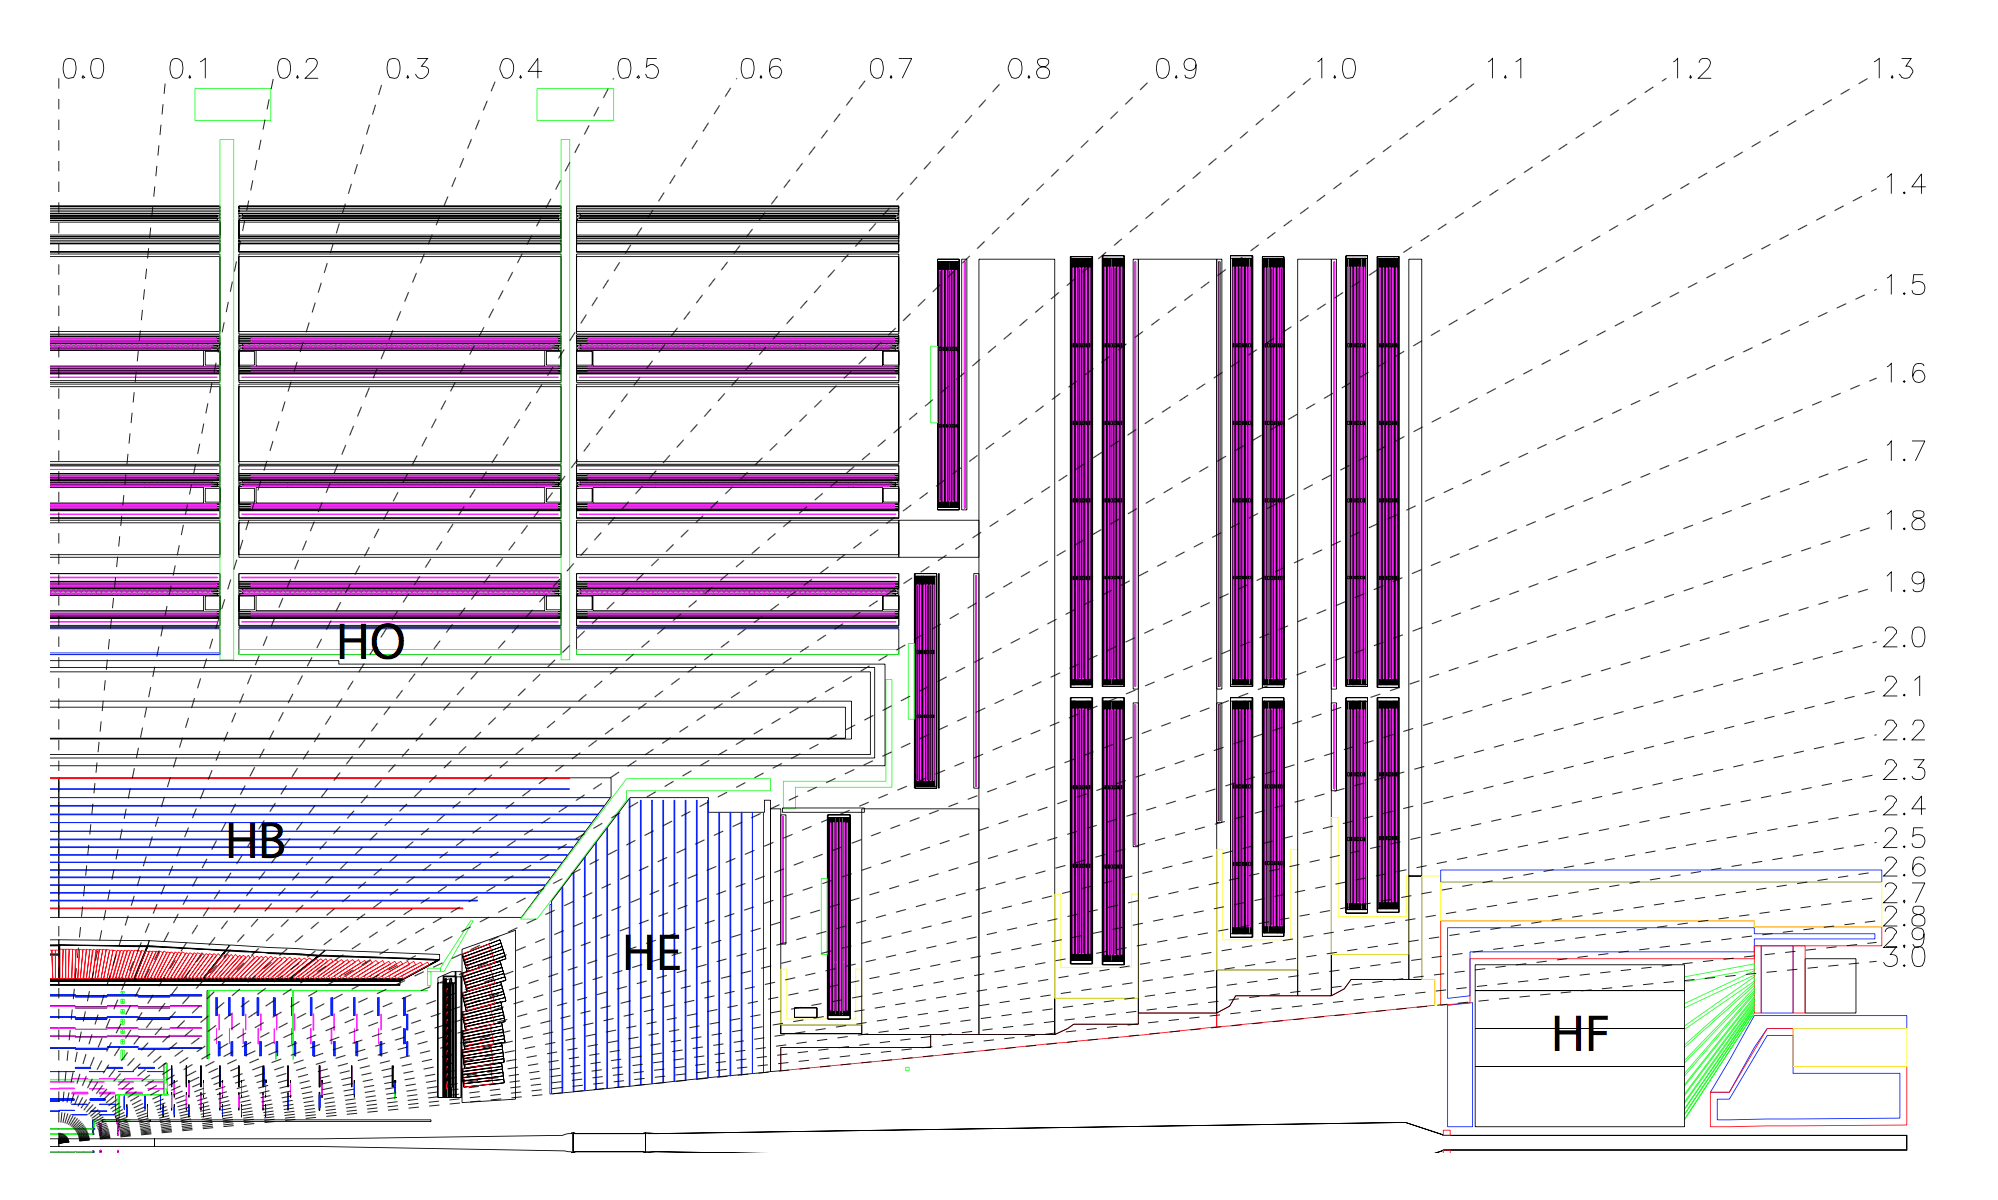
\includegraphics[width=0.9\textwidth]{./Detector/Plots/HCAL.png}
\caption{Illustration of the \ac{HCAL}, indicating the geometry
of the detector \cite{cms-jinst}.}
\label{fig:CMS_HCAL}
\end{center}
\end{figure}

The \ac{HB} and \ac{HE} are sampling calorimeters made of brass absorber
plates with tiles of plastic scintillator as the active material. The brass used as 
absorber fits the constraints imposed by the environment due to its short interaction length
of 16.42 cm and the fact that it is non-magnetic. The tiles of scintillator 
are $0.087 \times 0.087$ in $\eta-\phi$ for $|\eta|<1.6$ and $0.17\times0.17$ in $\eta-\phi$
beyond this range. 
The light from each tile is collected with a wavelength-shifting fibre, 
which is eventually read out using a hybrid photodiode. In the barrel, the \ac{HCAL}
has a thickness of between 5.82 and 10.6 interaction lenghts, which is not 
sufficient to identify for example late-starting showers. The \ac{HO}, sitting
outside of the magnet and using the coil as an additional absorber, extends the 
thickness to at least 11.8 interaction lenghts. 
The active material again consists of plastic scintillator tiles which roughly
map the granularity of the tiles in the \ac{HB}, read out by feeding the light
to a hybrid photodiode via wavelength shifting fibres.
%WTF: wavelength-shifting fibres

The \ac{HF}, providing coverage in the very forward region, is 
subjected to large radiation doses, requiring an extremely
radiation hard active material. For this reason quartz
fibres are used as active material. These fibres are embedded
in the steel absorber structure. Charged particles from the
shower initiated in the steel generate Cherenkov light in 
the quartz fibres, which is read out by photomultiplier tubes.
%Half of the fibres run over the full depth of the absorber
%while the other half starts at a depth of 22 cm, this is
%to distinguish electrons and photons (which deposit a large
%fraction of their energy in the first 22cm) from hadrons.

The energy resolution of the \ac{HCAL} for single charged pions 
was measured in a test beam \cite{cms-hcalecal}
and can be parameterised as 

\begin{equation}\label{eqn:hcal_res}
\frac{\sigma}{E} = \frac{S}{\sqrt{E}} \bigoplus C,
\end{equation}

where $S$ is the stochastic term, found to be 94.3\% %pm 1.2
and $C$ is the constant term, measured to be 8.4\% %pm 1.0
HCAL RESOLUTION!
%UPGRADE
During LS1, the \ac{HO} and \ac{HF} pmts were replaced 



\subsection{Muon system}
\label{sec:CMSLHC_CMS_muons}
One of the main physics goals of the \ac{CMS} experiment
at design was to search for $H\rightarrow ZZ\rightarrow 4\mu$ decays. Muons
suffer less from radiative losses in the tracker material, which means the most accurate
4-body mass can be constructed when using the dimuon final state of the $Z$'s.
Since the discovery of the Higgs boson the ZZ channel has continued to be an important
final state for Higgs measurements, at the same time many \ac{BSM} searches also make use of 
signatures with muons in the final state.
All of this means that good muon identification efficiency and precise muon momentum resolution
are very important. The \ac{CMS} muon system is made up out of three different subsystems which
are all necessary to ensure the identification requirements can be met. It is located
outside of the magnet coil, interspersed in the iron return yoke of the solenoid.
In the barrel of the detector the \ac{DT} chambers provide coverage for $|\eta|<1.2$, with
the \ac{CSC} covering the $0.9<|\eta|<2.4$ region. The \ac{RPCs}, covering the same
regions as both \ac{DT} and \ac{CSCs}, is used as a dedicated triggering system.

A cross-section of one quadrant of the detector, indicating
the positions of the \ac{DT},\ac{CSCs} and \ac{RPCs}, is shown in figure \ref{fig:CMS_MuonSystem}.
The top of the fourth muon endcap station as shown in this figure was added during \ac{LS1}, providing
additional layers of \ac{CSCs} and \ac{RPCs}.
\ac{LS1}.
\begin{figure}[h!]
\begin{center}
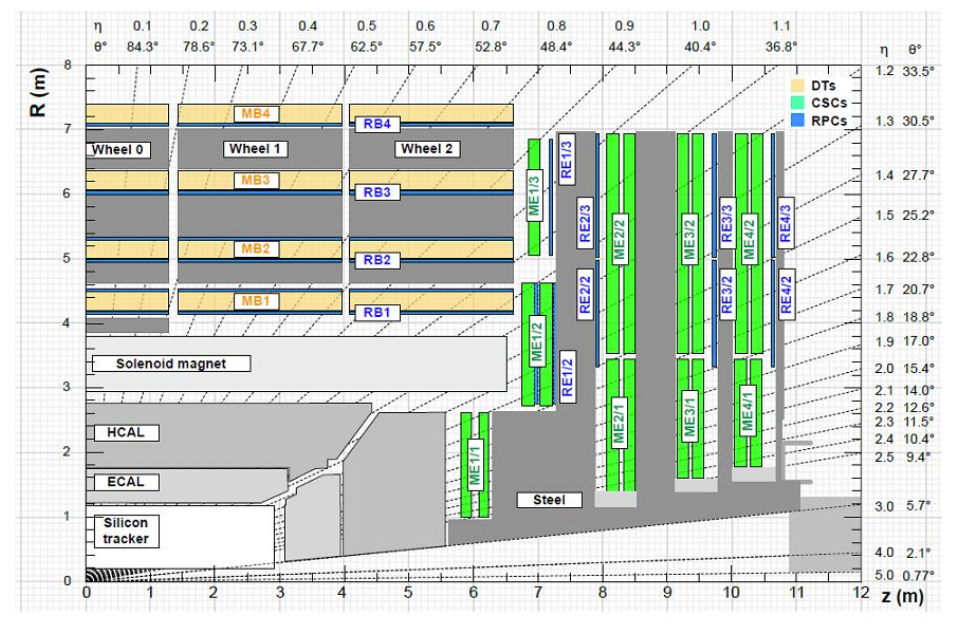
\includegraphics[width=0.8\textwidth]{./Detector/Plots/MuonSystemUpgrade.png}
\caption{Cross-section of one quadrant of the CMS detector, indicating
the positions of the different muon system components \cite{cms-muon-upgrade}. The 
fourth muon endcap stations were extended during \ac{LS1}, in Run 1 only the lower
part existed.}
\label{fig:CMS_MuonSystem}
\end{center}
\end{figure}

The \ac{DT} consists of layers of drift cells with a cross-section of $4.2 \times 1.3$ cm and
2.4 m long. The cells are filled with a mixture of %85\% 
Argon and carbon di-oxide gas.
Muons passing through the chamber ionise the gas, freeing electrons
which drift towards the anode wire running along the centre of the tube-shaped cell. 
This gives rise to an electric signal. There are 4 \ac{DT} stations in each wedge of 
the detector, each in turn consisting of 8 to 12 layers of drift tubes. Some of
these layers are oriented parallel to the beam line, providing a measurement of $\phi$.
There are also layers oriented orthogonal to the beam line, which give a measurement
of the z-coordinate. Measurements of the spatial resolution were made
during proton--proton running of the \ac{LHC} in 2010.
The spatial resolution of the \ac{DT} is 80-120 $\mu$m per chamber for
measurements in the $\phi$ direction, with the resolution of the $z$ measurement
is 130-400 $\mu$m\cite{cms-muon-7tev}.
%Drift lines distorted by magnetic field parallel to the wires

In the endcaps, where the muon rate is higher, the \ac{CSCs} provide
measurements of the muon track. These detectors are radiation-hard,
and have a fast response and fine segmentation.
Each of the CSC modules is a wedge-shaped
multi-wire proportional chamber %WTF
with 6 gaseous chambers bounded by cathode planes, with
sensitive strips placed on these plates in the
radial direction, to measure the coordinate in the  $r-\phi$ plane
of the muons. Anode wires in between the cathode planes
run along the $\phi$ direction and provide a measurement of
$\eta$. The resolution of the $r-\phi$ measurement is 40-120 $\mu$m \cite{cms-muon-7tev}.

In addition to the \ac{DT} and \ac{CSCs}, the \ac{RPCs} provide coverage
for $|\eta|<1.6$. These are made up of parallel plates, forming the anode and cathode,
with a gas gap in between. Ionisation of the gas due to the passing
muons is read out using aluminium strips running parallel to the 
beam axis. The position resolution of the \ac{RPCs} is much poorer than
that of the \ac{DT} and \ac{CSCs}, but their time response is very fast. As
a result of this the \ac{RPCs} can be used as an independent muon trigger
which can correctly identify the beam crossing from which the muon
originated.

To obtain precise muon momentum resolution, information from 
the tracker hits has to be combined with measurements in the
muon stations. The momentum resolution of the muon system
alone is 9\% for muons with \pT up to 200 GeV, and varies with $\eta$ 
between 15-40\% for muons with \pT of 1 TeV.


%Because of the uncertainty in the eventual background rates and in the ability of the muon system to measure the correct beam-crossing time when the LHC reaches full luminosity, a com- plementary, dedicated trigger system consisting of resistive plate chambers (RPC) was added in both the barrel and endcap regions. The RPCs provide a fast, independent, and highly-segmented trigger with a sharp pT threshold over a large portion of the rapidity range (|η| < 1.6) of the muon system. The RPCs are double-gap chambers, operated in avalanche mode to ensure good operation at high rates. They produce a fast response, with good time resolution but coarser position reso- lution than the DTs or CSCs. They also help to resolve ambiguities in attempting to make tracks from multiple hits in a chamber.

\subsection{Triggering and data processing}
\label{sec:CMSLHC_CMS_trigger}
When the \ac{LHC} is operating under standard conditions, protons are collided at a rate
of 40 MHz. This rate is too high for the \ac{DAQ} system to read out every event. In
addition this high collision rate produces such a large number of events that it would
not be feasible to write every single event, with sizes of around 1 MB, to tape. A trigger
system is therefore used to select events of interest for study, which reduces the rate
at which events are written to disk to  $\mathcal{O}(1 \text{ kHz})$.

The trigger system consists of two stages: the \ac{L1} trigger, which only makes use of
front-end electronics 
and reduces the event rate from 40 MHz to around 100 kHz, and the
\ac{HLT}, which runs on a computer farm with around 13000 CPU cores \cite{cms-trigger}.
During \ac{LS1} and the year-end technical stop at the end of 2015 the \ac{L1} trigger was
replaced by a completely upgraded system \cite{cms-trigger-tdr}, which provides amongst others 
improved object isolation, hadronic tau identification, muon \pT resolution and
jet finding with respect to the system used during Run 1.
An overview of the data flow in the \ac{L1} trigger is given in figure \ref{fig:CMS_Trigger}.

\begin{figure}[h!]
\begin{center}
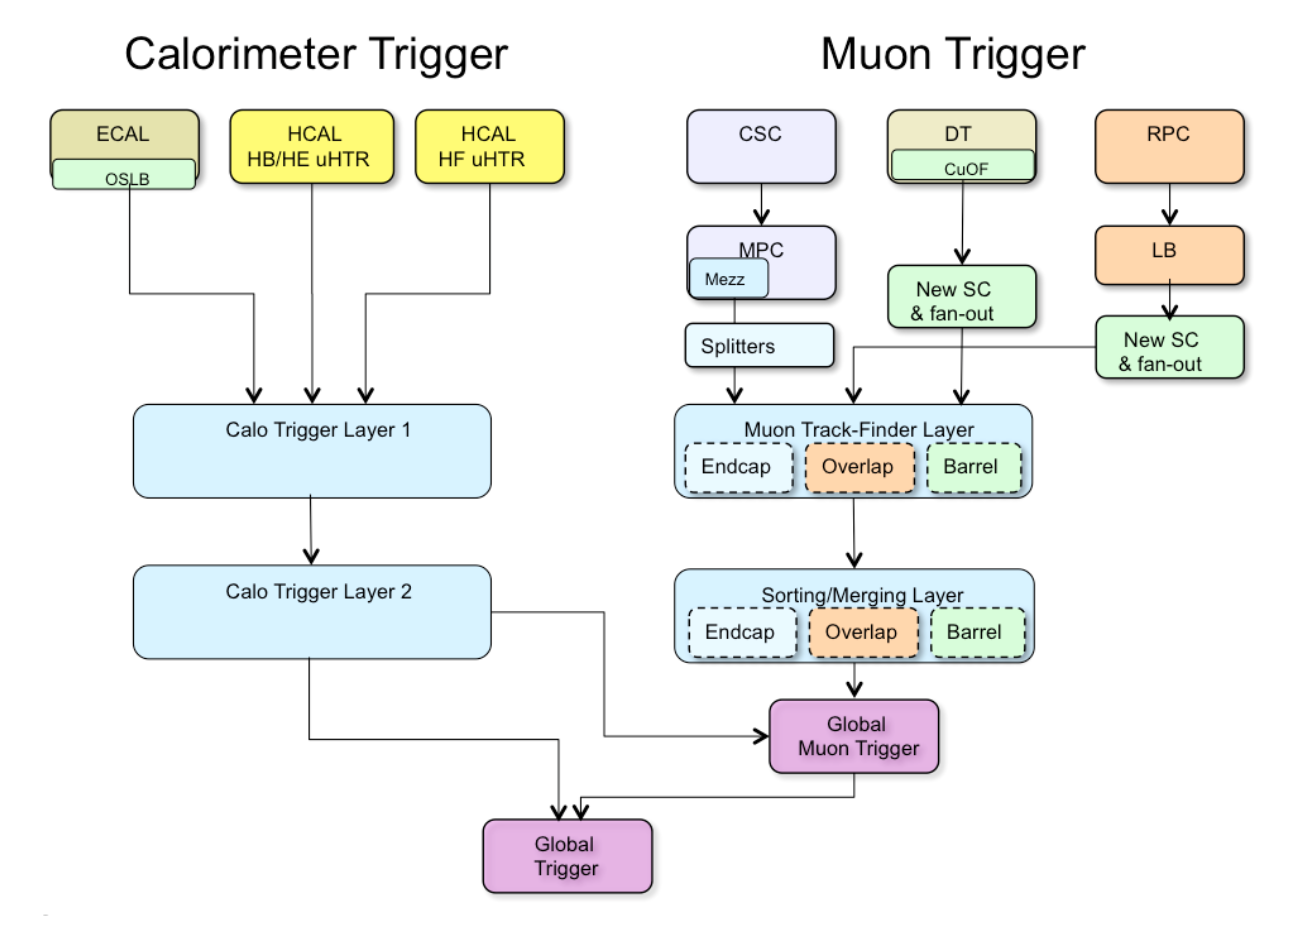
\includegraphics[width=0.5\textwidth]{./Detector/Plots/CMSTrigger.png}
\caption{Schematic of the different components of the \ac{L1} trigger \cite{cms-trigger-tdr}.}
\label{fig:CMS_Trigger}
\end{center}
\end{figure}


The \ac{L1} trigger only makes use of information from the calorimeters and the muon systems.
The calorimeter trigger starts from \ac{HCAL} and \ac{ECAL} energy deposits, 
which are fed to the first layer of the trigger. This layer maps onto
columns of the detector, receiving data from many bunch crossings. These data are passed
on to the second layer of the trigger in a way that bundles data from a single bunch crossing, but
different columns of the detector, to be processed on one node in the second layer of the
trigger. In this step basic object identification is performed based on the energy
deposits, so that a sorted list of the best candidates can be passed to the global trigger.
Hits in the muon chambers are read out and passed to the track finder layer 
of the muon trigger, which combines information from the \ac{CSC}, \ac{DT}
and \ac{RPC} systems in regions of $\eta-\phi$.
In further layers of the muon trigger the information from different
regions is combined, until finally the global muon trigger
can return a sorted list of the best muon candidates to the global trigger.
The global trigger combines the information from the calorimeter and muon triggers
to make a decision on whether the event should be sent to the \ac{HLT} or whether
it should be discarded. A decision has to be made within 3.2 $\mu s$, the maximum time during
which data can be stored in the front-end electronics before being lost.

%The muon trigger is a tracking trigger that measures the momentum of muons using the magnetic field in the steel yoke of the CMS solenoid; thus its resolution degrades with increasing momentum. This can be improved by maximizing the number of chamber hits along a muon trajectory and by improving the precision and number of position and angular measurements participating in the track fit applied in the trigger logic. Moreover, isolation criteria can be applied using the energy deposits in the calorimeter in order to further reduce the rate of muons from heavy flavor jets.

The \ac{HLT}, running on CPU nodes, makes use of the full information
from the detector, including tracker hits. This means particles
can be more accurately identified and their momentum is more
precisely known. The algorithms used in the \ac{HLT} are usually simpler
versions of those used in the full offline reconstruction. %Can't use full because time limited
During the 2012 run of the \ac{LHC} the \ac{HLT} operated with an output
capacity of around 1 kHz, for Run 2 this has increased. In August 2016, 
the \ac{HLT} output rate was 1.2 kHz for immediate data processing, with
an additional 0.6 kHz parked to be reconstructed and analysed when 
more processing power is available\cite{CMS-PAS-HIG-16-037}. %ie at the end of run 2

While the trigger system reduces the rate substantially, several
petabytes of data are produced by \ac{CMS} each year, in addition to 
even larger amounts of simulated datasets. To 
make these large amounts of data easily available for analysis, 
\ac{CMS} and the other \ac{LHC} experiments make use of the \ac{WLCG} \cite{lhc-wlcg}. 
The \ac{WLCG} pools the resources of computer centres at universities and research
laboratories around the world, based on a system of tiers. The Tier 0, at \ac{CERN} and
thw Wigner Research Centre for Physics in Budapest, performs the full reconstruction
and saves the data to tape. Datasets are copied to at least one Tier 1 centre, from
where data can be distributed to Tier 2 centres. The Tier 2 centres are located
at over 150 universities and research institutes around the world, providing 
resources for analysis of the datasets to all researchers associated with the experiment.



